\chapter{Deutch-Josza Algorithm}
\section{Problem}
Given a hidden boolean function $f$ acting on a string of bits, find out whether the function $f$ is a constant or balanced function. It is guaranteed that the function would definitely be one of these. 
\begin{equation}
\begin{split}
&\text{Constant: } f(\{x_0,x_1,x_2...\}) = 0 \text{ or } 1  \forall {x_0,x_1,x_2...} \in \{ 0,1\}^{\otimes n}\\
&\text{Balanced: } f(\{x_0,x_1,x_2...\}) = 0 \text{ half of the times and } 1 \text{ otherwise}
\end{split}
\end{equation}\section{Classical Solution}
In the worst case for the classical domain, we would have to check for half of the numbers plus one to determine if the function is balanced or not. So, if there are $n$ bits, a classical computer would take $2^{n-1}+1$ computations.\\
For this worst case to happen, we must get the same value for all the $2^{n-1} $ numbers we checked first. The probability of this happening is very low for the balanced case and often we can find that the function is balanced much earlier by using a randomized selection for numbers. but in the case of constant function, we would have to check for this many times to be 100\% sure. 
\section{Quantum Solution}

\begin{figure}[h]
\centering
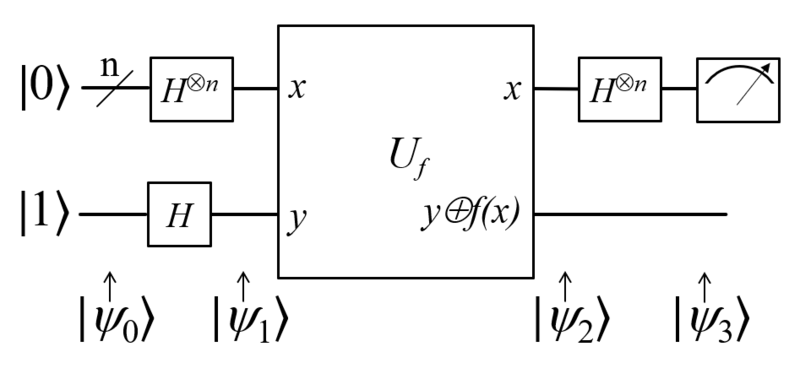
\includegraphics[width=0.5\textwidth]{images/dj.png}
\label{dj algo}
\caption{Circuit for Deutsch-Jozsa Algorithm}
\end{figure}
The above circuit can be used to solve the Deutsch-Jozsa Problem in one call only!!!\\
The function $U_f$ takes $|x\rangle |y\rangle$ and outputs $|x\rangle |y \oplus f(x)\rangle$. it is often referred to as \textit{Quantum Oracle} because we just assume we have such a gate without actually knowing $f$. Let us see what happens in this circuit:
\begin{enumerate}
\item We take the state $|\psi_0\rangle = |0\rangle ^{\otimes n} |1\rangle$ where the first $n$ bits act as the input register and last bit is used to store the result.
\item Apply Hadamard gate on all the bits. The state now becomes \begin{equation}
|\psi_1\rangle = \frac{1}{\sqrt{2^{n+1}}}\sum_{x=0}^{2^n -1} |x\rangle (|0\rangle - |1\rangle)
\end{equation}Here, the first $n$ bits are used to represent the number $x$.
\item Next, we apply the oracle on $|\psi_1\rangle$ to get \begin{equation} \begin{split}
|\psi_2\rangle &= \frac{1}{\sqrt{2^{n+1}}}\sum_{x=0}^{2^n -1} |x\rangle (|0 \oplus f(x)\rangle - |1 \oplus f(x)\rangle)\\
&= \frac{1}{\sqrt{2^{n+1}}}\sum_{x=0}^{2^n -1} (-1)^{f(x)} |x\rangle (|0 \rangle - |1 \rangle)
\end{split}
\end{equation}Notice that the last qubit value remains unchanged and the application of the quantum oracle actually changes the phase of the various values of the first register(the $|x\rangle$) depending on the value of $f(x)$.
\item Now, again apply the Hadamard gate but now only on the first register. Since there is no operation on the last qubit, it remains unchanged. So, we may focus on the values of the first register only.\begin{equation}
\begin{split}
|\psi_3\rangle_{register1} & = \frac{1}{2^{n}} \sum_{x=0}^{2^n -1} (-1)^{f(x)}  \left(\sum_{z=0}^{2^n-1} (-1)^{x.z} |z\rangle \right)\\
& = \frac{1}{2^{n}} \sum_{z=0}^{2^n -1} \left(\sum_{x=0}^{2^n-1} (-1)^{x.z + f(x)} \right)|z\rangle 
\end{split}
\end{equation}Notice that here, we have used the general form of Hadamard Gate :\begin{equation}
H^{\otimes n}|x\rangle= \frac{1}{\sqrt{2^n}}\left(\sum_{z=0}^{2^n-1} (-1)^{x.z} |z\rangle \right)
\end{equation}where $x.z = x_0z_0 \oplus x_1z_1 \oplus .. x_nz_n $ is the XOR of bit-wise product.(Verify this!!)
\item Lastly, we measure the value of first register. This will result in the collapsing of the first register in one of the states $|z\rangle$.
\begin{itemize}
\item If $f$ is a constant function, the coefficient of the state $|0\rangle^{\otimes n}$ is 1 or -1 depending on the value of $f(x)$. This means that the probability of measuring this state is 1. So, if the function is constant, we would observe the $|0\rangle^{\otimes n}$ state.
\item If $f$ is a balaced function, the coefficient of  the state $|0\rangle^{\otimes n}$ is 0 as $\sum(-1)^{x.0 + f(x)} = \sum(-1)^{f(x)} = 0 $ . So, there is zero probability of observing this state.
\end{itemize}
\end{enumerate}

Therefore by looking at the value of the first register, we can tell whether the function is constant or balanced.\\
This problem shows that quantum computer may offer an exponential speed over the classical computer. This is the case with other algorithms too.
